\chapter{NMR}
%************************************************

% \usepackage{amssymb}
%for making things bold easily, as we're working with a lot of vectors here
\def\*#1{\boldsymbol{#1}}
%for making unit vectors
\let\oldhat\hat
\renewcommand{\hat}[1]{\oldhat{\*{#1}}}

%for writing dual correspondance easily
\def\dc{\,\,\xleftrightarrow[\text{DC}]{}\,\,}
%for writing bras and kets
\def\bra#1{\langle#1|}
\def\ket#1{|#1 \rangle}
%inner product
\def\inpr#1#2{\langle #1|#2 \rangle}
%outer product
\def\oupr#1#2{| #1 \rangle \langle #2 |}
%bracket
\def\braket#1#2#3{\langle#1|#2|#3\rangle}
%hermitian adjoint
\def\ha#1{#1^\dagger}
%expectation value
\def\expval#1{\langle #1 \rangle}


\begin{flushright}
September 9 to 30, 2013 \\
% [$3 \times 6 hours spent$]
\end{flushright}


\section{$T_1$, $T_2$}
	\subsection{Minimal Introductory Theory}
		\subsubsection{Introduction}

		A nucleus of an atom has four intrinsic properties: Mass, electric
		charge, magnetic moment and the so called, `spin'. It is important
		to begin the discussion with the notion of quantization of angular
		momentum and then reconcile it with the idea of spin. For illustration,
		consider a rigid diatomic molecule rotating about some axis. This
		rotating molecule possesses a set of rotational states, in which the
		total angular momentum $L_{tot}$ has one of the following values:

		\begin{equation}
		L_\text{tot}=[J\ (J+1)]^{\frac{1}{2}}\hbar
		\end{equation}


		where J takes non negative integer values and $\hbar$ is the reduced
		Planck's constant. It is worth mentioning that the quantization is
		a condition on measurement and not a condition on existence. (Basically,
		$(1)$ gives a discrete set of eigenvalues for the angular momentum
		operator.) We might ask if there is any state for which $(1)$ doesn't
		hold; but that will be experimentally unobservable and hence irrelevant.
		Thus, $J$ completely determines the magnitude of the angular momentum
		for this system. However, in order to say something about the direction
		of rotation we need to introduce another quantum number $M_{J}$ where
		$M_{J}$ takes up $2\, J+1$ integer values from $-J$ to $J.$ In
		the absence of magnetic field, all these $2J\ +1$ states are degenerate.
		However, application of magnetic field breaks this degeneracy. This
		is called Zeeman effect. The energy separation between the $M_{J}$
		levels is termed as Zeeman splitting.

		Spin is also a kind of angular momentum, however, it is not produced
		due to the rotation of a particle, but is an intrinsic property of
		a particle, like mass and charge. Matter is built up in such a way
		that the spins of the different constituent particles cancel out in
		any large object. Thus, spin is not visible in the macroscopic world.
		It is precisely because of this reason that the concept of spin is
		very abstract and unintuitive; it doesn't have a classical analogue. 

		Spin angular momentum $S_{tot}$, is given by the following equation:

		\begin{equation}
		S_{tot}=[S\,(S+1)]^{\frac{1}{2}}\hbar
		\end{equation}


		Here again, $S$ can only take up a discrete set of values. For some
		particles, $S$ is a non negative integer while for some it is a half
		integer. The former are called bosons, the latter are named fermions.
		Thus, an elementary particle like an electron can two kinds of angular
		momentum; one arising from its motion whilst the other being its intrinsic
		property. $S$ for an electron is $\frac{1}{2}.$ 

		Now consider a system of two particles. The complete system has a
		total angular momentum quantum number given by either a sum of two
		individual angular momentum quantum numbers or their difference or
		any value in between. For example, consider two particles with spin
		2 and $\frac{1}{2}.$ The spin quantum number of the system can be
		$1\frac{1}{2},\ 2$ or $2\frac{1}{2}.$ Calculating spin for a system
		of more than two particles is more complicated. For the purpose of
		this experiment, it suffices to assume that there exists a certain
		way using which one can describe the spin of the nucleus as a whole.
		It is reasonable to guess that the total spin of zero corresponds
		to the state when there is an equal number of nucleons with opposite
		spin orientations. 


		\subsubsection{Nuclear spin}

		Protons and neutrons are made up of quarks. Both are spin $\frac{1}{2}$
		particles. Nuclear spin quantum number is denoted by $I$. Now, consider
		a proton in a nucleus with a mass number $M>1.$ The other nucleons
		can have their spin either parallel or anti-parallel to the first
		proton. Thus, there is a large number of configurations of spins of
		nucleons possible for a given nucleus. These nuclear states may have
		an enormous amount of energy difference among them ($\sim10^{11}kJ/mol$
		for $^{2}H)$. There are no simple rules to predict the ground state
		nuclear spin (the state with the lowest energy), however, a few guidelines
		are applicable:
		\begin{enumerate}
		\item If the no. of protons and neutrons are both even, the ground state
		nuclear spin is given by $I=0.$ 
		\item If the no. of protons and neutrons are both odd, the ground state
		nuclear spin is given by $I>0.$
		\end{enumerate}
		It is worth highlighting that the splitting between the nuclear ground
		state and the nuclear excited state is an entirely different phenomenon
		from the Freeman splitting. The former can be ignored in ordinary
		spectroscopy owing to the huge energy difference while the latter
		has magnitude far less than the thermal energies.


		\subsubsection{Microscopic magnetism and spin precession}

		Most of the macroscopic objects are observed to display an induced
		magnetism in the presence of an external field. The induced magnetic
		moment takes some time to build up. The equilibrium value of the magnetic
		moment is proportional to the external magnetic field.

		\begin{equation}
		\mu_{induced}=\mu_{0}^{-1}V\chi B
		\end{equation}


		Where $\mu_{0}$ is the permeability of the free space, V is the volume
		of the object and $\chi$ is a dimensionless quantity called the magnetic
		susceptibility expressing how readily the material develops the magnetic
		moment in the presence of magnetic field. $\chi$ can be negative
		as well, in which case the material is said to be diamagnetic. On
		the microscopic level, there are three fundamental sources of magnetism
		in an atom:
		\begin{enumerate}
		\item Circulation of electric current due to orbital motion of the electrons.
		\item Magnetic moments of the electrons.
		\item Magnetic moments of the nuclei.
		\end{enumerate}
		From Faraday's law (and Lenz' law), it can be guessed that the circulation
		of electric current contributes a negative value to the susceptibility,
		whilst the other two have positive contributions. In paramagnetic
		substances, i.e. the substances with positive $\chi$, the latter
		two contributions dominate over the first. A symmetry rule in quantum
		mechanics dictates that the spin and magnetic moment operator have
		the following relation:

		\begin{equation}
		\hat{\mu}=\gamma\hat{S}
		\end{equation}


		For a nucleus, $\gamma$ is called the gyromagnetic ratio, different
		for different isotopes. Now, consider a macroscopic bar magnet in
		an external magnetic field $B.$ The magnet has a magnetic moment
		$\mu$ along its axis. In this scenario, the tendency of the bar magnet
		is to rotate and orient itself in the parallel (or anti-parallel)
		to the direction of the applied magnetic field. However, $(4)$ gives
		rise to a whole new phenomenon in case of quantum particles like nuclei.
		In this case, there is a precession of angular momentum (and thus,
		magnetic moment) around the direction of applied magnetic field. Thus
		spin polarization (direction of spin angular momentum) sweeps a cone
		around the magnetic field, keeping a constant angle between the spin
		magnetic moment and the field that depends only on the initial spin
		polarization. The frequency of this precession is proportional to
		the external magnetic field. 

		\begin{equation}
		\omega^{0}=-\gamma B^{0}
		\end{equation}


		Where $\omega^{0}$ is called the Larmor frequency. The frequency
		is considered positive according to the right hand thumb rule convention,
		where thumb points in the direction of $B$. 


		\subsubsection{Spin-lattice relaxation}

		Spin orientations of nuclei of a typical sample, e.g. $H$ nuclei
		in water, are uniformly distributed in all the directions, the total
		magnetic moment being very close to zero. In the presence of a magnetic
		field, all the nuclei begin executing Larmor precession. However,
		the atoms which contain these nuclei are undergoing `collisions' with
		each other. This thermal motion hence, gives rise to slight fluctuations
		in the magnetic fields that the nuclei experience. At any given time,
		the local magnetic field experienced by anyone nuclear spin is slightly
		different, both in magnitude and direction to its neighbour. These
		small fluctuating fields due to neighbouring atoms cause a gradual
		breakdown of constant angle `cone precession' of the nuclear spins.
		Over a long period of time, the magnetic moment of each nuclear spin
		wanders around, moving between different `precession cones' and eventually
		sampling the entire range of possible orientations.The time scale
		of precession motion is a few nanoseconds whilst that of the wandering
		motion can be as large as a second. The thing to notice is this that
		since the environment has some temperature, it is slightly more probable
		that the nuclear spin is driven towards an orientation with higher
		magnetic energy. This anisotropy of the magnetization distribution
		in thermal equilibrium means that the entire sample acquires a small
		net magnetic moment along the field, i.e. a longitudinal magnetic
		moment. It is found that:

		\begin{equation}
		\chi_\text{nuc}=\frac{\mu_{0}\hbar^{2}\gamma^{2}c}{4k_{b}T}
		\end{equation}


		Where $c$ is the number of protons per unit volume. Assume that the
		magnetic moment at equilibrium is denoted by $M_{eq}^\text{nuc}.$ Magnetic
		moment of the material after time $t$ of application of magnetic
		field to the sample can be approximated by the following relation:

		\begin{equation}
		M_{z}(t)=M_\text{eq}(1-e^{\frac{-t}{T_{1}}})
		\end{equation}


		In the above expression, $T_{1}$is the time constant called the spin-lattice
		relaxation time constant which depends on the isotope, viscosity and
		temperature etc.


		\subsubsection{Spin-Spin relaxation}

		The longitudinal nuclear spin magnetization is too weak to be of any
		experimental importance. The following technique is employed. Suppose
		that the spin system is allowed to reach a thermal equilibrium, on
		microscopic level which corresponds to a large number of nuclear spin
		magnets precessing around the magnetic field at the same frequency
		. Let us choose a rectangular coordinate system such that the applied
		field is in z-direction. There is no net magnetization in the transverse
		directions. Suppose now an r.f. pulse is applied to the system such
		that all the spin orientations are rotated by $\frac{\pi}{2}$ to,
		say $x-$ directions. Once the pulse is removed, all the nuclei begin
		to precess around $z-$ axis at an angle of $\frac{\pi}{2}$. The
		net magnetic moment perpendicular to the field applied is called the
		transverse magnetization. It should be noted that this transverse
		magnetization will decay with the passage of time because the spin
		polarizations will cease to precess in synchrony. The factors responsible
		for making the precession out of sync are lack of homogeneity in
		the applied magnetic fields, fluctuations in the field due to thermal
		motion etc. Macroscopic magnetizations at a time $t$ after the pulse
		has been applied has the form:

		\begin{equation}
		\begin{array}{c}
		M_{y}=-M_\text{eq}^\text{nuc}cos(\omega_{0}t)e^{\frac{-t}{T_{2}}}\\
		M_{x}=M_\text{eq}^\text{nuc}sin(\omega_{0}t)e^{\frac{-t}{T_{2}}}
		\end{array}
		\end{equation}
		It should be noted that there is an exponential decay with a time
		constant $T_{2.}$ This decay constant is termed as the transverse
		relaxation time constant. It so happens that this rotating magnetic
		field produces an electric field according to the Faraday's law. If
		a wire loop is placed at a suitable location near the changing magnetic
		field, then the electrons of the wire can be brought into motion.
		Thus a tiny current is generated which can be detected. 


		\subsubsection{NMR Signal}

		The oscillating current in the previous expression is called the \emph{NMR signal}
		or \emph{free-induction decay}. This NMR signal has the information about
		the Larmor frequency and the time constants.


	\subsection{Instrumentation Setup}
		On a broad level, an NMR spectrometer extracts information about a
		given sample in three steps. 
		\begin{enumerate}
		\item Allowing the magnetic nuclear spins in the samples to reach thermal
		equilibrium in a large homogeneous magnetic field.
		\item Rotating the nuclear spin polarizations by an r.f. pulse.
		\item Detecting and amplifying the weak r.f. signals that is emitted as
		the spins resume their precession motion in the magnetic field. 
		\end{enumerate}
		This poses certain challenges on the machinery. Firstly, the NMR signal
		is very weak. Secondly the NMR frequencies must be measured with extremely
		high accuracies. Thus there are twin challenges of sensitivity and
		resolution. The spectrometer has following parts:


		\subsubsection{Magnet}

		In order to avoid inhomogeneous broadening, the spectrometer uses a
		magnetic field with extremely high homogeneity ($1$ part in $10^{9}$).
		The NMR spectrometer in the lab employs the use of superconducting
		magnets. The magnetic field it can produce is of the magnitude 14.7
		T. This corresponds to a Larmor frequency of 600 MHz for a TMS Hydrogen.
		Maintain the superconducting coils (made up of an alloy of Nb and
		Sn) at a low temperature requires a constant cooling by a bath of
		liquid helium. The liquid helium bath is itself insulated by another
		large reservoir of liquid nitrogen. Through the centre of the large
		cylindrical can of coolant and the superconducting coils there is
		a large cavity (insulated from the magnets) called bore. The sample
		is placed on a probe and kept inside the bore so that it experiences
		the highest magnetic field. The temperature inside the bore can be
		brought to the room temperature. There are two additional sets of
		coils called shims. There are two kinds of them: one wound from superconducting
		material immersed in the liquid helium bath, called superconducting
		shims and the other supported on a tube that is inserted into the
		magnet bore, called the room temperature shims. Shims act as a correction
		for the inhomogeneity of the magnetic field.


		\subsubsection{The Transmitter Section}

		This is the part of the spectrometer that produces the r.f. irradiation.
		In our instrument there were four transmitter sections each dedicated
		to producing r.f. signals at frequencies close to the Larmor frequencies
		of different isotopes: $C^{13},\ H,\ F$ and $D.$ In general the
		synthesizer output wave of a transmitter section is given by 
		\begin{equation}
		s_\text{synth}\sim cos(\omega_\text{ref}t\ +\phi(t))
		\end{equation}


		Here $\phi(t)$ is the r.f. phase while the term $t$ is the time
		coordinate. In general, this term $\phi(t)$ jumps rapidly between
		different values, the discontinuous phase jumps being controlled by
		a timing device called the pulse programmer. In general, we need only
		a short pulse of r.f. and hence it is important to chop out a `time-slice'
		of the r.f. waveform. This is done by the pulse gate. The duration
		of an r.f. pulse is termed as the pulse width. Finally, a radio frequency
		amplifier is used to scale up the gated and shifted waveform so as
		to produce a large amplitude r.f. pulse. 


		\subsubsection{The Duplexer}

		The amplified r.f. pulse goes to the probe via duplexer. Another cable
		emanates from the duplexer which goes to the receiver section. The
		role of the device is two fold. It makes sure that the pulse from
		the transmitter section goes only to the probe and not to the the
		sensitive receiver section. Secondly, the tiny NMR signal goes only
		to the receiver and not to the transmitter section. There are multiple
		ways of doing this but the electronics behind the Duplexer is beyond
		the scope of this report. 


		\subsubsection{The Probe}

		The probe has several functions:
		\begin{enumerate}
		\item Locating the sample in a region of homogeneous magnetic field.
		\item Exposing the sample to r.f. waves, detecting the r.f. emissions from
		the sample.
		\item Maintaining the temperature of the sample.
		\item Rotating the sample to reduce broadening. (at a frequency of around
		10 Hz)
		\item Using \emph{cryoprobes} to reduce the temperature of electronic circuits
		to improvise signal detection.
		\item Creating controlled inhomogeneity in magnetic field, often needed
		in diffusion related and imaging experiments.
		\end{enumerate}

		\subsubsection{The Receiver Section}

		The receiver section consists of various sub-parts, the first of which
		is the signal pre-amplifier, responsible for amplifying the r.f. emission
		from the sample. Secondly, the quadrature receiver combines the NMR
		signal, which oscillates at the Larmor frequency $\omega_{ref}$,
		with the reference signal, oscillating at the frequency $\omega^{0}$,
		to generate a new signal that oscillates at the relative Larmor frequency
		$\Omega=\omega^{0}-\omega_{ref}$. This is done because for computer
		analysis, one needs to convert the incoming waveform into a digital
		signal. However, the present ADC converters can't handle such a high
		frequency and the latter needs to be brought down, a job accomplished
		by the quadrature receiver. 


	\subsection{Theory}
		\subsubsection{Prerequisites}
			For this section, it is recommended that chapters 10, 11 and 12 are read from Levitt. However, only the following concepts (for spin $1/2$ particles) are required for a working knowledge of the experiments.

			\begin{enumerate}
				\item Law of motion of a spin particle under a constant magnetic field and the associated rotation matrices and angular momentum operators
				\item Concept of a rotating frame and the transformed Hamiltonian
				\item Equation of motion for precession in the rotating frame
				\item Effect of an RF pulse on the Hamiltonian \label{singleSpinRF} *
				\item Understanding of effect of specific pulses like $(\pi/2)_X$ on the spin particle's state ket
				\item Effect of a generalized pulse on the state ket and nutation (a qualitative picture would suffice)
				\item Density operator; its need, significance and definition
				\item For a spin 1/2 system; the physical significance of the terms of the density operator and order of coherence
				\item Derivation of the density operator at thermal equilibrium
				\item Density operator in the rotating frame
				\item Associated to the density operator, the magnetization vector
				\item Effect of an RF (strong) pulse on the density operator (using the definition and \autoref{singleSpinRF}) *
				\item Effect of specific pulses like $(\pi/2)_X$ and $(\pi)_X$ (coherence excitation and population inversion)
				\item Free precession without relaxation
				\item Phenomenological understanding of transverse and longitudinal relaxation
				\item Measurement of $T_1$ using population inversion and coherence *
				\item Measurement of $T_2$ using Spin Echo *
			\end{enumerate}

			The starred concepts have been discussed in some detail in this report. The notation is identical to that used in Levitt and the meaning of the symbols may be implied from the context.

		\subsubsection{Effect of an RF pulse on the Hamiltonian}
			When an RF pulse is applied, the spin particle experiences two magnetic fields, one being the static magnetic field and the other being the oscillating field from the excitation coil. The RF pulse is much weaker than the static magnetic field, but is resonant to the precession frequency of the spin particle. As time goes on, the weak RF field brings about a large change in the spin state.


			When an RF pulse of phase $\phi_p$ along the x-axis of the fixed reference system. The oscillations of the RF pulse oscillating at the spectrometer reference frequency $\omega_\text{ref}$, can be described as the two components rotating in the opposite frequency viz the resonant component rotating in the same sense as the nuclear spin precession, while the non-resonant component rotating in the opposite. 

			Neglecting the non-resonant component, the spin hamiltonian during an RF pulse
			\begin{equation}
			\hat{{H}} = \omega^0 \hat{I_z} + \hat{{H}}_\text{RF}(t)
			\end{equation}

			where 
			\begin{equation}
			\hat{{H}}_\text{RF}(t) \approx - \frac{1}{2} \gamma B_\text{RF} \sin \theta_\text{RF} { \cos ( \omega_\text{ref}t + \phi_p) \hat{I}_x + \sin ( \omega_\text{ref}t + \phi_p) \hat{I}_y } 
			\end{equation}

			Apply the sandwich relation to obtain

			\begin{equation}
			\hat{{H}}_\text{RF}(t) \approx - \frac{1}{2} \gamma B_\text{RF} \sin \theta_\text{RF} \hat{R}_z(\Phi_p) \hat{I}_x \hat{R}_z(-\Phi_p) 
			\end{equation}

			where 
			\begin{equation}
			 \Phi_P(t) = \omega_\text{ref} t + \phi_P
			\end{equation}


			In rotating frame, the spin Hamiltonian is given by a
			\begin{equation}
				\hat{ {H}}  = \hat{R}_z (-\Phi) \hat{{H}} \hat{R}_z (\Phi) - \omega_\text{ref}\hat{I}_z
			\end{equation}

			Applying this, we obtain
			\begin{equation}
			\hat{{{H}}} = - \frac{1}{2} \gamma B_\text{RF} \sin \theta_\text{RF} \hat{R}_z (-\Phi + \Phi_p) \hat{I}_x \hat{R}_z (\Phi - \Phi_p) + (\omega^0 -\omega_\text{ref}) \hat{I}_z
			\end{equation}

			where 
			\begin{equation}
			\Phi (t) = \omega_\text{ref} t + \phi_\text{ref} 
			\end{equation}

			Finally, upon substitution, we obtain
			\begin{equation}
			\hat{{{H}}} \approx - \frac{1}{2} \gamma B_\text{RF} \sin \theta_\text{RF} \hat{R}_z (-\phi_\text{ref} + \phi_p) \hat{I}_x \hat{R}_z (\phi_\text{ref} - \phi_p) + \Omega^0 \hat{I}_z
			\end{equation}

			where $\Omega^0$ is the resonance offset.
			As is visible, there is no time dependence in the expression.

			We can also substitute for $\phi_\text{ref}$, for positive spins it equals $\pi$,


			\begin{equation}
			\hat{{{H}}} \approx \omega_\text{nut} \hat{R}_z (\phi_p) \hat{I}_x \hat{R}_z (-\phi_p) + \Omega^0 \hat{I}_z
			\end{equation}

			where the nutation frequency $w_\text{nut}$ is given by, 
			\begin{equation}
			\omega_\text{nut} = \| \frac{1}{2} \gamma B_\text{RF} \sin \theta_\text{RF} \|
			\end{equation} 

			Applying the sandwich relation again, 

			\begin{equation}
			\hat{{{H}}} \approx \Omega^0 I_z + \omega_\text{nut}(\hat I_x \cos \phi_p + I_y \sin \phi_p)
			\end{equation}

		% \subsubsection{Effect of an RF (strong) pulse on the density operator}
		% 	Prashansa's doing it
		\subsubsection{Phenomenological understanding of transverse and longitudinal relaxation}
			We know the thermodynamically stable populations of a given spin $\frac 1 2$ ensemble. If this population distribution is disturbed, then the system is restored to the equilibrium distribution eventually. This effect is known as longitudinal relaxation, and $T_1$ quantifies this behaviour.

			Similarly, at equilibrium, the coherence is zero. If coherence is introduced, it gradually dies out. This is the transverse relation which is quantified by $T_2$.

			For $T_1$, we have the following phenomenological equations.
			\begin{align}
				\rho_{\alpha 3} &= (\rho_{\alpha 2} - \rho_{\alpha}^\text{eq})e^{-\tau/T_1} + \rho_{\alpha}^\text{eq} \\
				\rho_{\beta 3} &= (\rho_{\beta 2} - \rho_{\beta}^\text{eq})e^{-\tau/T_1} + \rho_{\beta}^\text{eq} \\
				\text{where  } \rho_{\alpha}^\text{eq}&=\frac 1 2 + \frac 1 4 \mathbb B \\
							\rho_{\beta}^\text{eq}&=\frac 1 2 - \frac 1 4 \mathbb B
			\end{align}

			$T_1$ is typically in the range $100 ms$ - $100 s$.

			For $T_2$, we have the following equations that describe the phenomenon.
			\begin{align}
				\rho_{-3} &= \rho_{-2} e^{(i\omega^0 - \lambda)\tau} \\
				\rho_{+3} &= \rho_{+2} e^{(-i\omega^0 - \lambda)\tau}\\
				\text{where } \lambda &= T_2^{-1}
			\end{align}
			We performed an experiment to find $\lambda$, as will be discussed in the next sections.

			The precise mechanisms of this process has not been dealt with here and only a phenomenological explanation is provided. However, physically one can think of it as follows. On an average the magnetic field (say along $\hat z$ is constant) is constant and at an instant $t_0$ the spins are synchronised. However, there always exist some local fluctuations due to the environment of each individual spin which leads to loss of synchronization, and consequently coherence.

		\subsubsection{Measurement of $T_1$ using population inversion and coherence}
			Consider the pulse sequence $\pi_X \;\; \tau \;\; \pi/2_X$ which is repeated for different values of $\tau$ on a given sample and the data is collected for a fixed $t$. The resulting NMR data can be represented using a 2D data matrix = $S(\tau,t)$.
			Before proceeding further, some subtleties have been listed
			\begin{enumerate}
				\item In the actual experiment, the acquisition is repeated to reduce errors
				\item Each acquisition is separated by time $\tau_\text{wait}$ to allow the sample to return to thermal equilibrium. ($\tau_\text{wait}$ and $\tau$ should be much greater than $T_1$)
				\item Something known as a phase cycle is also performed, but has been ignored here (as was done in Levitt, in this discussion)
			\end{enumerate}
			Let us now look at what the pulse sequence is really doing and then we'll come to the NMR data and its rudimentary analysis. The action of the pulses on the density operator has been re-written for reference.
			\begin{itemize}
				\item $\pi_X$ generates an inverted population distribution
				\item $\pi/2_X$ converts the population difference into coherence, including the observable (-1)-quantum coherence.
			\end{itemize}
			In terms of the density operator, we can represent the action of the pulse sequence as
			\begin{align}
				\hat \rho_1  &= \hat \rho_\text{eq} = \frac 1 2  \hat 1 + \frac 1 2 \mathbb B \hat I_z \\
				\hat \rho_2  &= R_x(\pi) \hat \rho_1 R_x(-\pi) \\
						&= \frac 1 2 \hat 1 - \frac 1 2 \mathbb B \hat I_z \\
				\hat \rho_3  &= \frac 1 2 \hat 1 + \frac 1 2 \mathbb B (1-2 e^{-\tau/T_1})\hat I_z \\
				\hat \rho_4	&= R_x(\pi/2) \hat \rho_3 R_x(-\pi/2) \\
						&= \frac 1 2 \hat 1 - \frac 1 2 \mathbb B (1 - 2 e^{-\tau/T_1}) \hat I_y
			\end{align}
			The NMR signal then becomes
			\begin{align}
				S(\tau,t) &=a(\tau)e^{(i\omega^0 - \lambda)t} \\
				\text{where   } a(\tau)&=\frac 1 2 \mathbb B(1-2e^{-\tau/T_1})
			\end{align}
			If we plot $a(\tau)$ vs $\tau$, we expect the graph to start with a negative $Y$ intercept, and monotonically rising and then asymptotically stabilizing at $y=\frac 1 2 \mathbb B$.
		\subsubsection{Measurement of $T_2$ using Spin Echo}
			$T_2$ as was described physically earlier, arises from the de synchronization of spins which leads to loss of coherence. We therefore first investigate the concept of peak broadening which is essential to understand the need of spin echo in the first place.

			Peak broadening is caused primarily be two factors which are called
			\begin{enumerate}
				\item Homogeneous: This arises due to microscopic magnetic fluctuations (quantified by $T_2$).
				\item Inhomogeneous: This is caused by the strong `macroscopic' magnetic field's inhomogeneity (which is with great pain, attempted to be as homogeneous as possible)
			\end{enumerate}
			If there were no inhomogeneous broadening, we could easily measure $T_2$ from the peak broadening. However, there still is a way known as spin echo that can cleverly, selectively measure homogeneous decay, allowing for the measurement of $T_2$.


			Let us look understand inhomogeneous broadening in a little more depth. Figure 12.6 (from Livett) illustrates how multiple spins, when slightly out of phase, cancel out the effect spin, resulting in a sharper decline, and thus a larger peak width.

			In the frequency domain, there are many peaks centred around the the peak, which cause the broadening.

			We are now ready to discuss the spin echo pulse sequence, the heart of the experiment. The pulse sequence used is $\pi/2_X \; \tau/2 \; \pi_Y \; \tau/2$ as is given in figure 12.7 of the text. Let's start as usual with the thermal equilibrium state.
			\begin{align}
				\rho_1 = \rho^\text{eq} &= \frac 1 2 \hat 1 + \frac 1 2 \mathbb B \hat I_z\\
				\rho_2 &= \frac 1 2 \hat 1 - \frac 1 2 \mathbb B \hat I_y
			\end{align}
			From this point onwards, no other pulse converts the populations to coherences, thus the $\hat 1$ term will be dropped (as it doesn't contribute to the NMR signal).
			\begin{align}
				\rho_3 &= \frac 1 2 \mathbb B (-\hat I_y \cos(\omega^0 \frac 1 2 \tau) + \hat I_x \sin(\omega^0 \frac 1 2 \tau) e^{-\lambda \frac 1 2 \tau} + ...	\\
				\rho_4 &= \frac 1 2 \mathbb B (-\hat I_y \cos(\omega^0 \frac 1 2 \tau) - \hat I_x \sin(\omega^0 \frac 1 2 \tau) e^{-\lambda \frac 1 2 \tau} + ... \\
				\rho_5 &= - \frac 1 2 \mathbb B \hat I_y e^{-\lambda \tau}
			\end{align}
			And from the last step, we know the peak amplitude in the NMR spectrum will be
			\begin{align}
				a(\tau)=\frac 1 2 \mathbb B e^{-\lambda \tau}
			\end{align}
			Do you see the brilliance of the result? Note that the final density operator is independent of $\omega^0$! Which means that the signal is independent of the (inhomogeneity) applied magnetic field and we have successfully found a way of determining $\lambda$.

			However, we can gain more insight into this mechanism by geometric considerations; by just staring at figure 12.14 - 12.16.
	\subsection{Practical Implementation}
		\begin{enumerate}
			\item Loading the sample
				\begin{enumerate}
					\item Ejected the existing item on the air cushion
					\item Loaded the sample using the stairs
				\end{enumerate}
			\item NMR operation using TopSpin \\
				Following is a summary of the commands executed to obtain the data. The pulse sequences were changed in accordance with the experiment ($T_1$ $T_2$). We were assisted by a PhD student at the NMR lab, with the performance of the experiment.
				\begin{enumerate}
					\item check no acquisition running
					\item \texttt{ebc}:
					experiment number, title, check solvent used(we use acetone with D), lock field
					\item \texttt{rsh}:
					command for shimming which is done artificially using standard samples by making fields homogenous with respect to them and using them as reference.
					\item \texttt{getprosol}:
					command for retreiving the values of parameters like pulse, duration, delays, aquisition time etc.
					\item \texttt{lock}:
					command to select solvent, we used AcetoneD6
					\item \texttt{atma}:
					automatic tuning matching automatically 
					\item \texttt{atmm}:
					automatic tuning matching manually 
					\item \texttt{rga}:
					receiver gain automatic
					\item \texttt{rgm}:
					reciever gain manual
					\item \texttt{zg}:
					sets the pulse program t1ir1D, with D1=20s
					\item \texttt{starts acquiring FID}:
					\item \texttt{efp }:
					command to perform experimental fourier transformation 
					\item \texttt{apk}:
					automatic phase correction
					\item \texttt{abs}:
					automatic baseline correction, it can be done manually too using the command `absm'
				\end{enumerate}
			\end{enumerate}

	\subsection{Observations}
		Upon analysis of the existing experimental data, $T_1$ was found to be $7.43 \pm 0.060 (0.81\%)$ for the first and $7.92 \pm 0.059 (0.74\%)$ seconds for the second peak, with the corresponding graphs, \autoref{e3T1P1} and \autoref{e3T1P2} and data, \autoref{e3T1}. We further found $T_2$ to be $78.055 \pm 5.739 (7.35\%)$ for the first and $84.762 \pm 5.613 (6.22\%)$ seconds for the second peak. The corresponding graphs are given in \autoref{e3T2P1} and \autoref{e3T2P2} with the corresponding data in \autoref{e3T2}. 
		\par
		It is surprising however that we obtained $T_2>T_1$ while the theoretic limit is $2T_1>T_2$, which lead us to the implication that the data we analysed was for two different compounds.
		\par
		The data corresponding to our experiment was lost before it could be recovered from the NMR machine.

		\lstinputlisting{gfx/T1}\label{e3T1}
		\lstinputlisting{gfx/T2}\label{e3T2}

		\begin{figure}[bth]
			\begin{center}
				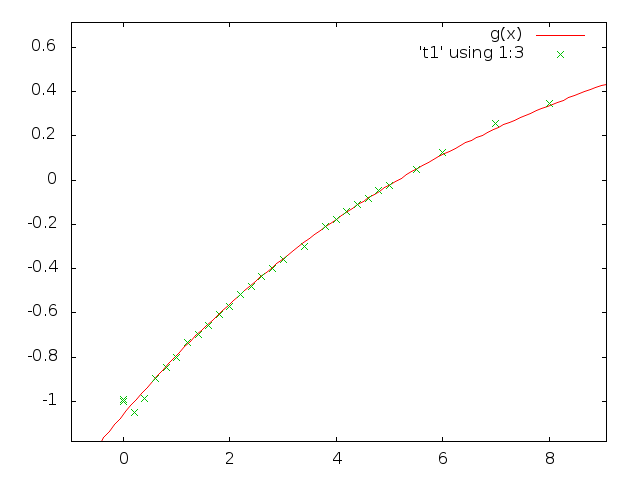
\includegraphics[width=1.1\linewidth]{gfx/e3_T1P1}
			\end{center}
		\caption[$T_1$, peak 1]{Intensity vs Time (sec), for $T_1$, peak 1}
		\label{e3T1P1}
		\end{figure}

		\begin{figure}[bth]
			\begin{center}
				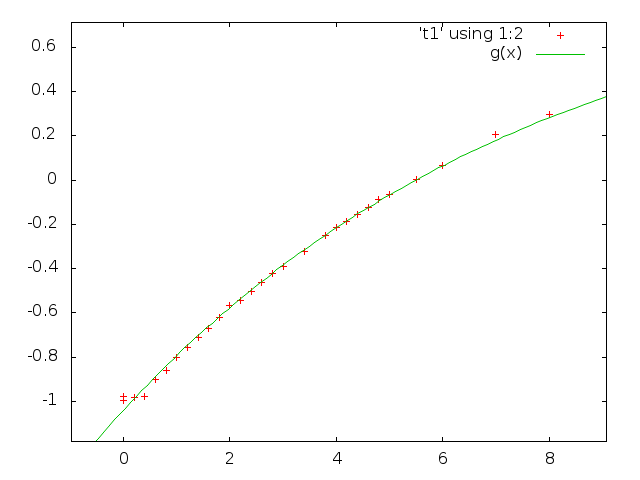
\includegraphics[width=1.1\linewidth]{gfx/e3_T1P2}
			\end{center}
		\caption[$T_1$, peak 2]{Intensity vs Time (sec), for $T_1$, peak 2}
		\label{e3T1P2}
		\end{figure}

		\begin{figure}[bth]
			\begin{center}
				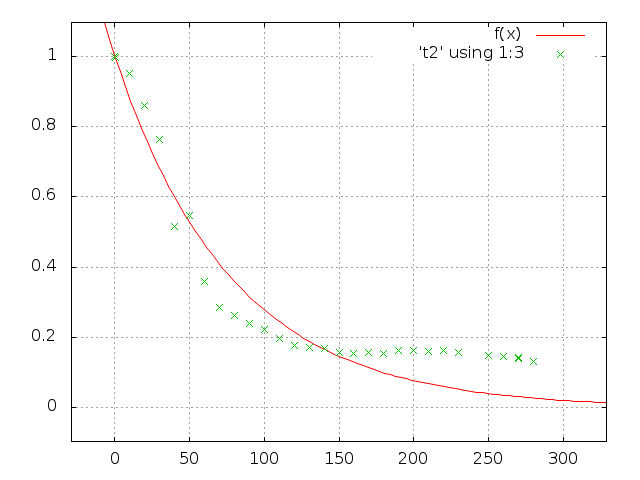
\includegraphics[width=1.1\linewidth]{gfx/e3_T2P1}
			\end{center}
		\caption[$T_2$, peak 1]{Intensity vs Time, for $T_2$, peak 1}
		\label{e3T2P1}
		\end{figure}

		\begin{figure}[bth]
			\begin{center}
				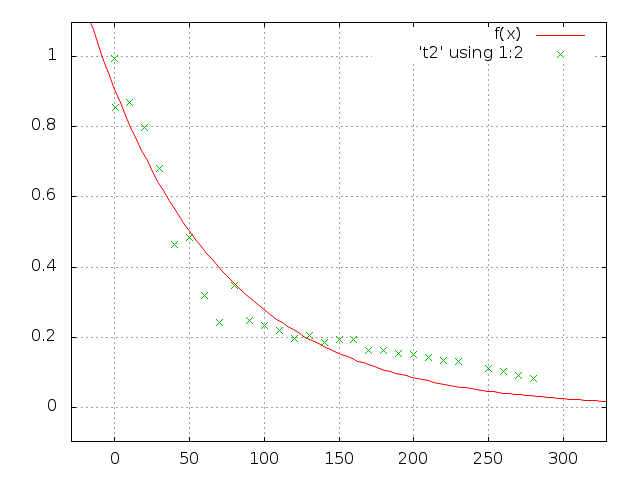
\includegraphics[width=1.1\linewidth]{gfx/e3_T2P2}
			\end{center}
		\caption[$T_2$, peak 2]{Intensity vs Time, for $T_2$, peak 2}
		\label{e3T2P2}
		\end{figure}


\section{Diffusion}
	There are two important things to understand in this experiment.
	\begin{itemize}
	\item The phenomenon of diffusion and Einstein-Stokes' equation.
	\item Pulse Field Gradient - Spin Echo (or PFGSE)
	\end{itemize}

	\subsection{Theory}
		Diffusion is the random translational (or Brownian) motion of molecules
		or ions across a system driven by its internal thermal energy. Translational
		diffusion is the basic mechanism by which molecules are distributed
		in space and plays an important role in any chemical reaction. The
		systems for which there is an initial concentration gradient, Fick's
		laws quantitatively explains the relation between the (instantaneous
		and local) concentration and the flux of the molecules/ions.

		Fick's first law postulates that the flux of a material across a given
		plane is proportional to the concentration gradient across the plane.
		In other words,

		\begin{equation}
		J\ =-D\frac{\partial C(x,t)}{\partial x}
		\end{equation}


		Where \emph{J} is the flux (Number/meter$^{2}$ sec) and \emph{$\frac{\partial C(x,t)}{\partial x}$}
		is the concentration gradient. The constant of proportionality is
		called the diffusion constant and has the dimensions of $length^{2}/time$.
		There is a negative sign to show that molecules/ions are flowing in
		the direction of lower concentration. The above postulate is sufficient
		to understand the behaviour of the systems for which the concentration
		gradient doesn't vary with time. To analyse the variations in concentration
		due to time, Fick further postulated that the magnitude of change
		in the local concentration over time is equal to that in local diffusion
		flux, implying,

		\begin{equation}
		\frac{\partial C(x,t)}{\partial t}=-\frac{\partial J(x,t)}{\partial x}
		\end{equation}


		The above two equations can be combined to give the one dimensional
		version of the famous diffusion (or heat) equation:

		\[
		\frac{\partial C(x,t)}{\partial t}=\frac{\partial^{2}C(x,t)}{\partial x^{2}}
		\]


		It is assumed that the diffusion coefficient is independent of the
		position. There are three more things to be proven before one can
		move on to the NMR concepts. Firstly, The mean square value of the
		displacement of the particles can be evaluated as $6Dt.$ To prove
		this, one first needs to find the fundamental solution of the diffusion
		equation. Let us skip the long procedure of deriving the fundamental
		solution of the diffusion equation and take it as:

		\begin{equation}
		P(x,t)=\frac{1}{(\sqrt{4\pi D})^{3}}e^{\frac{-(x-x_{0})^{2}}{4Dt}}
		\end{equation}


		Average of any function $L(t)$ can now be calculated as:

		\begin{equation}
		<L(t)>\equiv\int_{\mathbb{R}^{3}}L(x,t)P(x,t)dx
		\end{equation}


		Secondly, we need Stoke's law that the force needed to move a small
		sphere of radius \emph{R} through a continuous medium of viscosity
		$\eta$ with a velocity \emph{V} is given by the following relation:

		\begin{equation}
		F=6\pi\eta RV
		\end{equation}


		Lastly, Einstein-Stoke's equation describes the way that diffusion
		increases in proportion to temperature, and is inversely proportional
		to the frictional force experienced by a molecule $f,$ where $f=6\pi\eta R.$
		Thus, 
		\begin{equation}
		D=\frac{k_{B}T}{6\pi\eta R}
		\end{equation}


	\subsection{Practical Implementation}
		In this section we discuss the `Pulse Field Gradient - Spin Echo' technique.

		Let's take a detour and first understand what spin echo sequence means.
		Imagine that one has a sample where initially the magnetization of
		the molecules is parallel to the external field. 
		% Let's ignore the diffusion effects for a while. 

		A $90^o$ pulse is applied along the x direction so that
		the net magnetization now lies in the xy plane, in the y axis. During
		the period of time following the removal the RF pulse, each spin experiencing
		a slight variation in magnetic field begin to fan out slowly or \textquotedblleft{}dephase\textquotedblright{}.
		The variations in the magnetic field come from both transverse relaxation
		due to T$_{2}$ (spin-spin interaction) and inhomogeneities in the
		external field. The importance of the spin echo experiment is that
		the effects of the inhomogeneities are made reversible. At a time
		$\tau$ a $180$º pulse is applied along the y direction. The spins
		are therefore rotated by $180^o$ around the y axis thereby
		remaining in the xy plane. As a result of the inverted relative positions,
		and because each spin continues to precess with its former frequency,
		all spins will be perfectly re-clustered at time $2\tau$ forming what
		is called an echo.%
		\footnote{Diffusion measurements by NMR, http://www.uni-muenster.de/%
		}

		How are this de-phasing and echoing related to diffusion coefficient
		measurements? Well, imagine now that I have the sample enclosed in
		a thin tube. If I apply an external magnetic field that varies linearly
		with height then I should expect a linear variation in the larmor
		frequencies. Heterogeneous magnetic field is often supplied by applying
		two pulses of duration $\delta$ and constant gradient $g$ between
		the $90$º and $180\text{º}$ pulse and after the $180$º pulse with
		an interval of time $\Delta$ between them, in the background of a
		homogeneous field. If the molecules are now in translational motion
		then the re-phasing of the spins won't be perfect as the frequency
		of the spin vector while de-phasing is different from the frequency
		while re-phasing. This decreases the intensity of the spin echo which
		can be quantified by the following expression:

		\begin{equation}
		I(t)=e^{-\frac{2\tau}{T_{2}}}e^{-Dg^{2}\gamma^{2}\delta^{2}(\Delta-\delta/3)}
		\end{equation}\label{diffusionEquation}

		We can vary $I$ by keeping any $2$ quantities out of $g,\ \delta,\ \Delta$
		constant and varying one and do a best fit with equation $7$ to obtain
		$D.$ In our experiment we varied $g$ and held all the other parameters
		constant. 

	\subsection{Observations and Result}
		The data obtained has been listed in \autoref{e3diffusionData}, where the first column is the percentage of gradient strength, the following columns represent the intensity of two different peaks. Only the first has been used for further analysis in the report.
		Experimentally, $\delta = 800 \mu s = 8\times 10^{-4}s, \Delta=15 ms=1.5\times10^{-2}s,g=( \text{fraction}) \times 53.5 \times 0.63 G cm^{-1}= () 33.7\times 10^4 Tcm^{-1}, \gamma = 2.675 222 \times 10^8 s^{-1}T^{-1}$ and plugging them into \autoref{diffusionEquation} and taking log on both sides, we get 
		\begin{align}
			\log I &= \text{const} - D\times(7809.87)\times(\text{gradient intensity fraction})^2 \\
					&= \text{const} - D\times(0.780987)\times(\text{GPZ6})^2
		\end{align}
		Upon curve fitting, we get 
		\begin{equation}
			D\times(0.780987)=-0.000154109 \pm 2.209\times 10^{-7} (0.1433\%)
		\end{equation}
		from which we get $D=1.973\times 10^{-4} (\pm 0.1433\%) cm^2 s^{-1}$
		\lstinputlisting{gfx/diffusion}\label{e3diffusionData}

		% % GNUPLOT: LaTeX picture
\setlength{\unitlength}{0.240900pt}
\ifx\plotpoint\undefined\newsavebox{\plotpoint}\fi
\begin{picture}(1500,900)(0,0)
\sbox{\plotpoint}{\rule[-0.200pt]{0.400pt}{0.400pt}}%
\put(130.0,82.0){\rule[-0.200pt]{4.818pt}{0.400pt}}
\put(110,82){\makebox(0,0)[r]{-0.2}}
\put(1419.0,82.0){\rule[-0.200pt]{4.818pt}{0.400pt}}
\put(130.0,179.0){\rule[-0.200pt]{4.818pt}{0.400pt}}
\put(110,179){\makebox(0,0)[r]{ 0}}
\put(1419.0,179.0){\rule[-0.200pt]{4.818pt}{0.400pt}}
\put(130.0,276.0){\rule[-0.200pt]{4.818pt}{0.400pt}}
\put(110,276){\makebox(0,0)[r]{ 0.2}}
\put(1419.0,276.0){\rule[-0.200pt]{4.818pt}{0.400pt}}
\put(130.0,373.0){\rule[-0.200pt]{4.818pt}{0.400pt}}
\put(110,373){\makebox(0,0)[r]{ 0.4}}
\put(1419.0,373.0){\rule[-0.200pt]{4.818pt}{0.400pt}}
\put(130.0,471.0){\rule[-0.200pt]{4.818pt}{0.400pt}}
\put(110,471){\makebox(0,0)[r]{ 0.6}}
\put(1419.0,471.0){\rule[-0.200pt]{4.818pt}{0.400pt}}
\put(130.0,568.0){\rule[-0.200pt]{4.818pt}{0.400pt}}
\put(110,568){\makebox(0,0)[r]{ 0.8}}
\put(1419.0,568.0){\rule[-0.200pt]{4.818pt}{0.400pt}}
\put(130.0,665.0){\rule[-0.200pt]{4.818pt}{0.400pt}}
\put(110,665){\makebox(0,0)[r]{ 1}}
\put(1419.0,665.0){\rule[-0.200pt]{4.818pt}{0.400pt}}
\put(130.0,762.0){\rule[-0.200pt]{4.818pt}{0.400pt}}
\put(110,762){\makebox(0,0)[r]{ 1.2}}
\put(1419.0,762.0){\rule[-0.200pt]{4.818pt}{0.400pt}}
\put(130.0,859.0){\rule[-0.200pt]{4.818pt}{0.400pt}}
\put(110,859){\makebox(0,0)[r]{ 1.4}}
\put(1419.0,859.0){\rule[-0.200pt]{4.818pt}{0.400pt}}
\put(130.0,82.0){\rule[-0.200pt]{0.400pt}{4.818pt}}
\put(130,41){\makebox(0,0){ 0}}
\put(130.0,839.0){\rule[-0.200pt]{0.400pt}{4.818pt}}
\put(261.0,82.0){\rule[-0.200pt]{0.400pt}{4.818pt}}
\put(261,41){\makebox(0,0){ 1000}}
\put(261.0,839.0){\rule[-0.200pt]{0.400pt}{4.818pt}}
\put(392.0,82.0){\rule[-0.200pt]{0.400pt}{4.818pt}}
\put(392,41){\makebox(0,0){ 2000}}
\put(392.0,839.0){\rule[-0.200pt]{0.400pt}{4.818pt}}
\put(523.0,82.0){\rule[-0.200pt]{0.400pt}{4.818pt}}
\put(523,41){\makebox(0,0){ 3000}}
\put(523.0,839.0){\rule[-0.200pt]{0.400pt}{4.818pt}}
\put(654.0,82.0){\rule[-0.200pt]{0.400pt}{4.818pt}}
\put(654,41){\makebox(0,0){ 4000}}
\put(654.0,839.0){\rule[-0.200pt]{0.400pt}{4.818pt}}
\put(784.0,82.0){\rule[-0.200pt]{0.400pt}{4.818pt}}
\put(784,41){\makebox(0,0){ 5000}}
\put(784.0,839.0){\rule[-0.200pt]{0.400pt}{4.818pt}}
\put(915.0,82.0){\rule[-0.200pt]{0.400pt}{4.818pt}}
\put(915,41){\makebox(0,0){ 6000}}
\put(915.0,839.0){\rule[-0.200pt]{0.400pt}{4.818pt}}
\put(1046.0,82.0){\rule[-0.200pt]{0.400pt}{4.818pt}}
\put(1046,41){\makebox(0,0){ 7000}}
\put(1046.0,839.0){\rule[-0.200pt]{0.400pt}{4.818pt}}
\put(1177.0,82.0){\rule[-0.200pt]{0.400pt}{4.818pt}}
\put(1177,41){\makebox(0,0){ 8000}}
\put(1177.0,839.0){\rule[-0.200pt]{0.400pt}{4.818pt}}
\put(1308.0,82.0){\rule[-0.200pt]{0.400pt}{4.818pt}}
\put(1308,41){\makebox(0,0){ 9000}}
\put(1308.0,839.0){\rule[-0.200pt]{0.400pt}{4.818pt}}
\put(1439.0,82.0){\rule[-0.200pt]{0.400pt}{4.818pt}}
\put(1439,41){\makebox(0,0){ 10000}}
\put(1439.0,839.0){\rule[-0.200pt]{0.400pt}{4.818pt}}
\put(130.0,82.0){\rule[-0.200pt]{0.400pt}{187.179pt}}
\put(130.0,82.0){\rule[-0.200pt]{315.338pt}{0.400pt}}
\put(1439.0,82.0){\rule[-0.200pt]{0.400pt}{187.179pt}}
\put(130.0,859.0){\rule[-0.200pt]{315.338pt}{0.400pt}}
\put(1279,819){\makebox(0,0)[r]{'diffusion' using ($1*$1):(log($2))}}
\put(1311,179){\makebox(0,0){$+$}}
\put(1076,313){\makebox(0,0){$+$}}
\put(866,431){\makebox(0,0){$+$}}
\put(683,538){\makebox(0,0){$+$}}
\put(526,628){\makebox(0,0){$+$}}
\put(395,702){\makebox(0,0){$+$}}
\put(290,763){\makebox(0,0){$+$}}
\put(212,807){\makebox(0,0){$+$}}
\put(1349,819){\makebox(0,0){$+$}}
\put(1279,778){\makebox(0,0)[r]{g(x)}}
\multiput(1299,778)(20.756,0.000){5}{\usebox{\plotpoint}}
\put(1399,778){\usebox{\plotpoint}}
\put(212,807){\usebox{\plotpoint}}
\put(212.00,807.00){\usebox{\plotpoint}}
\put(229.94,796.58){\usebox{\plotpoint}}
\put(248.00,786.37){\usebox{\plotpoint}}
\put(265.82,775.75){\usebox{\plotpoint}}
\put(284.10,765.95){\usebox{\plotpoint}}
\put(301.99,755.46){\usebox{\plotpoint}}
\put(320.21,745.52){\usebox{\plotpoint}}
\put(337.98,734.83){\usebox{\plotpoint}}
\put(356.20,724.87){\usebox{\plotpoint}}
\put(373.98,714.19){\usebox{\plotpoint}}
\put(392.01,703.91){\usebox{\plotpoint}}
\put(410.23,693.97){\usebox{\plotpoint}}
\put(428.00,683.27){\usebox{\plotpoint}}
\put(446.18,673.25){\usebox{\plotpoint}}
\put(464.00,662.64){\usebox{\plotpoint}}
\put(482.05,652.42){\usebox{\plotpoint}}
\put(500.20,642.40){\usebox{\plotpoint}}
\put(518.19,632.06){\usebox{\plotpoint}}
\put(536.21,621.79){\usebox{\plotpoint}}
\put(554.06,611.23){\usebox{\plotpoint}}
\put(572.21,601.16){\usebox{\plotpoint}}
\put(590.00,590.50){\usebox{\plotpoint}}
\put(608.14,580.46){\usebox{\plotpoint}}
\put(626.20,570.25){\usebox{\plotpoint}}
\put(644.01,559.63){\usebox{\plotpoint}}
\put(662.20,549.62){\usebox{\plotpoint}}
\put(679.97,538.93){\usebox{\plotpoint}}
\put(698.36,529.32){\usebox{\plotpoint}}
\put(716.19,518.72){\usebox{\plotpoint}}
\put(734.39,508.75){\usebox{\plotpoint}}
\put(752.18,498.08){\usebox{\plotpoint}}
\put(770.27,487.92){\usebox{\plotpoint}}
\put(788.18,477.45){\usebox{\plotpoint}}
\put(806.30,467.33){\usebox{\plotpoint}}
\put(824.37,457.13){\usebox{\plotpoint}}
\put(842.20,446.53){\usebox{\plotpoint}}
\put(860.25,436.30){\usebox{\plotpoint}}
\put(878.20,425.89){\usebox{\plotpoint}}
\put(896.13,415.46){\usebox{\plotpoint}}
\put(914.41,405.68){\usebox{\plotpoint}}
\put(932.26,395.11){\usebox{\plotpoint}}
\put(950.41,385.05){\usebox{\plotpoint}}
\put(968.19,374.35){\usebox{\plotpoint}}
\put(986.41,364.41){\usebox{\plotpoint}}
\put(1004.18,353.72){\usebox{\plotpoint}}
\put(1022.62,344.19){\usebox{\plotpoint}}
\put(1040.40,333.51){\usebox{\plotpoint}}
\put(1058.17,322.81){\usebox{\plotpoint}}
\put(1076.40,312.88){\usebox{\plotpoint}}
\put(1094.17,302.18){\usebox{\plotpoint}}
\put(1112.37,292.20){\usebox{\plotpoint}}
\put(1130.42,281.95){\usebox{\plotpoint}}
\put(1148.50,271.78){\usebox{\plotpoint}}
\put(1166.41,261.32){\usebox{\plotpoint}}
\put(1184.37,250.94){\usebox{\plotpoint}}
\put(1202.41,240.69){\usebox{\plotpoint}}
\put(1220.47,230.47){\usebox{\plotpoint}}
\put(1238.65,220.46){\usebox{\plotpoint}}
\put(1256.43,209.77){\usebox{\plotpoint}}
\put(1274.35,199.32){\usebox{\plotpoint}}
\put(1292.43,189.13){\usebox{\plotpoint}}
\put(1310.23,178.49){\usebox{\plotpoint}}
\put(1311,178){\usebox{\plotpoint}}
\put(130.0,82.0){\rule[-0.200pt]{0.400pt}{187.179pt}}
\put(130.0,82.0){\rule[-0.200pt]{315.338pt}{0.400pt}}
\put(1439.0,82.0){\rule[-0.200pt]{0.400pt}{187.179pt}}
\put(130.0,859.0){\rule[-0.200pt]{315.338pt}{0.400pt}}
\end{picture}

		\begin{figure}[bth]
			\begin{center}
				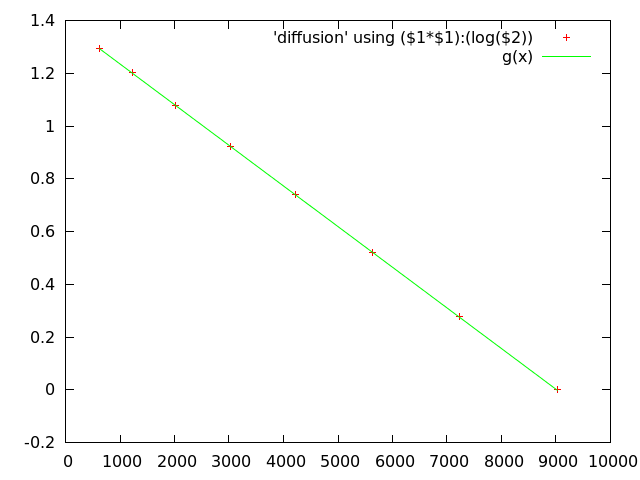
\includegraphics[width=1.1\linewidth]{gfx/diffusionGraph}
			\end{center}
		\caption[log(Intensity) vs Gradient Percentage$^2$]{For diffusion, log(Intensity) vs Gradient Percentage$^2$}
		\label{e3diffusion}
		\end{figure}

	% \subsection{Understanding the Pulse Business}
	% 	\subsubsection{Notation and the spin 1/2 system}
	% 		Let $\ket{\alpha}$ and $\ket{\beta}$ represent the two eigenvectors of the $I_z$ angular momentum operator. So in general the system can be in a state $\ket\psi$ given by
	% 		\begin{equation}
	% 			\ket{\psi}=c_\alpha \ket{\alpha} + c_\beta \ket{\beta}
	% 		\end{equation}
	% 		where $c_\alpha$ and $c_\beta$ are complex numbers. Further we also have $\inpr{\psi}{\psi}=1$.

	% 		Thus accordingly we have in this basis of the eigenkets of $I_z$,
	% 		\begin{equation}
	% 		{			
	% 			\ket\alpha \doteq
	% 			\left(
	% 			\begin{array}{c}
	% 				1 \\
	% 				0 \\
	% 			\end{array}
	% 			\right)
	% 		}
	% 		\end{equation}

	% 		\begin{equation}
	% 		{			
	% 			\ket\beta \doteq
	% 			\left(
	% 			\begin{array}{c}
	% 				0 \\
	% 				1 \\
	% 			\end{array}
	% 			\right)
	% 		}
	% 		\end{equation}
	% 		For easy refernce, the Angular Momentum operators have also been given in their matrix representation with respect to this basis.
	% 		\begin{equation}
	% 		{			
	% 			I_z \doteq
	% 			\frac{1}{2}
	% 			\left(
	% 			\begin{array}{cc}
	% 				1 & 0 \\
	% 				0 & -1 \\
	% 			\end{array}
	% 			\right)
	% 		}
	% 		\end{equation}
	% 		\begin{equation}
	% 		{			
	% 			I_y \doteq
	% 			\frac{1}{2i}\left(
	% 			\begin{array}{cc}
	% 				0 & 1 \\
	% 				1 & 0 \\
	% 			\end{array}
	% 			\right)
	% 		}
	% 		\end{equation}
	% 		\begin{equation}
	% 		{			
	% 			I_x \doteq
	% 			\frac{1}{2}\left(
	% 			\begin{array}{cc}
	% 				0 & 1 \\
	% 				1 & 0 \\
	% 			\end{array}
	% 			\right)
	% 		}
	% 		\end{equation}

	% 		In general, we can create an ket $\ket{\theta,\phi}$ \footnote{Here $\theta$ is the angle of the vector from the $+Z$ axis and $\phi$ is the azimuthal angle measured from $+X$} in arbitrary direction which is an eigenket of the momentum operator in that direction.
	% 		\begin{equation}
	% 			\ket{\theta,\phi} \doteq \left( 
	% 			\begin{array}{c}
	% 				\cos{\theta/2} e^{-i\phi/2} \\
	% 				\sin{\theta/2} e^{+i\phi/2} \\
	% 			\end{array}
	% 			\right)
	% 		\end{equation}
	% 		with the operator given by
	% 		\begin{equation}
	% 			I_{\theta,\phi} = I_z \cos \theta + I_x \sin \theta \cos \phi + I_y \sin \theta \sin \phi
	% 		\end{equation}
	% 		such that
	% 		\begin{equation}
	% 			I_{\theta,\phi} \ket{\theta,\phi}= +\frac 1 2 \ket{\theta,\phi}
	% 		\end{equation}

	% 	\subsubsection{Law of Motion}
	% 		The Law of motion for a time independent
	% 		\begin{equation}
	% 			a=a
	% 		\end{equation}